\section{Zielsetzung}
Ziel dieses Versuches ist es, den Photoeffekt zu untersuchen und den Zusammenhang zwischen 
Elektronenenergie und Wellenlänge mithilfe der Elektroquantendynamik zu erklären.

\section{Theorie}
\label{sec:Theorie}
Der Photoeffekt beschreibt die Auslösung von Elektronen aus einer Metalloberfläche, welche mit Licht
bestrahlt wird. Dabei treten Effekte auf, die mit der klassischen Physik nicht zu erklären sind und quantenmechanisch
erklärt werden müssen.
Generell wird zur Beobachtung des Photoeffekts eine Photozelle wie in \autoref{fig:Photozelle} verwendet. Einfallende Photonen
lösen aus der Oberfläche der Photokathode Elektronen aus. Zwischen der Photokathode und der Auffängerelektrode lässt sich eine
Spannung $U_{\symup{B}}$ anlegen, mit der die ausgelösten Elektronen abgebremst werden können, sodass sich die Energie der Elektronen
über die Gegenfeldmethode bestimmen lässt. Darüber hinaus wird der Photostrom $I$ mithilfe eines Picoamperemeters gemessen.
\begin{figure}[H]
    \centering
    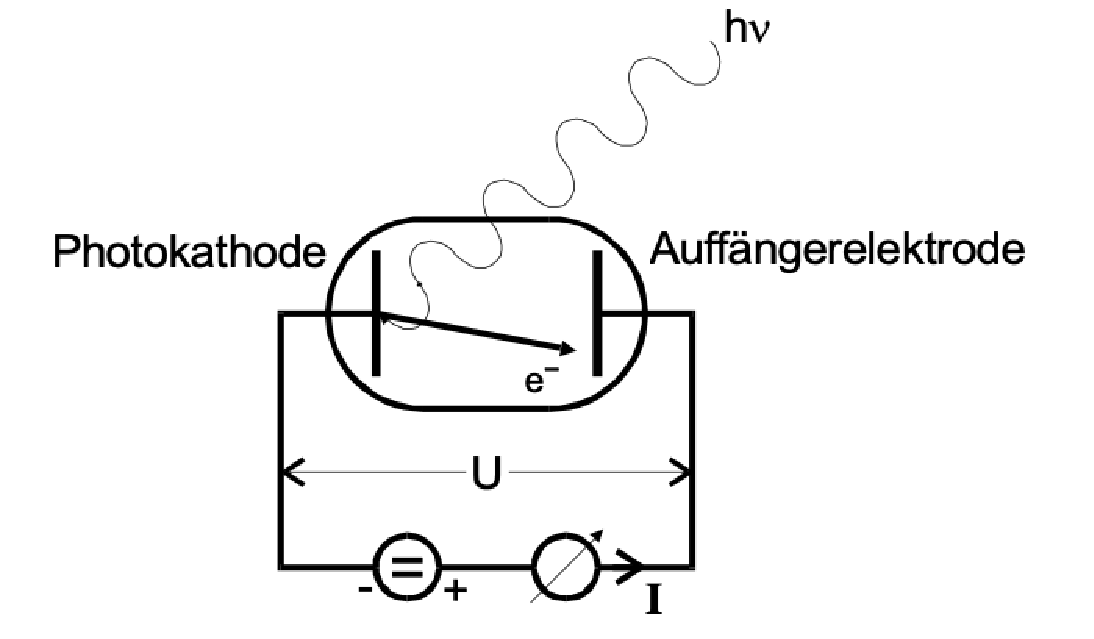
\includegraphics[height=6cm]{content/pics/Photozelle.pdf}
    \caption{Schematische Darstellung einer Photozelle \cite{v500}.}
    \label{fig:Photozelle}
\end{figure}

\subsection{Beschreibung von Licht}
In der Historie wurden vor allem zwei Theorien verwendet, um die Eigenschaften und Effekte von Licht zu beschreiben. Nach der 
\textbf{korpuskularen Theorie} wird Licht als sehr kleines Teilchen betrachtet, wohingegen Licht in dem \textbf{Wellenmodell}
als Welle aufgefasst wird.

Die Auslösung von Photoelektronen nach dem Wellenmodell ließe sich so erklären, dass Elektronen durch konstruktive Interferenz Energie
gewinnen und so die Bindungsenergie zum Atom überwinden.
Da die Resonanzkatastrophe nicht unmittelbar eintreten kann, wird erwartet, dass der Photostrom verzögert einsetzt. Es wird jedoch 
beobachtet, dass Elektronen sofort ausgelöst werden.
Außerdem wäre zu erwarten, dass die Energie der Photoelektronen mit der Intensität des Lichtes zunimmt. Tatsächlich wird beobachtet, dass
nicht die Energie, sondern die Anzahl der Photoelektronen (Photostrom $I$) mit der Intensität steigt.
Das Wellenmodell lässt auch den Schluss zu, der Photostrom steige mit der Frequenz des Lichtes, da so mehr Elektronen gelöst würden. 
Beobachtet wird hingegen ein Anstieg der Energie der Elektronen.

Diese Erkenntnisse stehen folglich im direkten Widerspruch zu dem Wellenmodell. In anderen Experimenten, wie etwa dem Doppelspaltexperiment,
wird wiederum widerlegt, dass Licht im klassichen Sinn aus Korpuskeln besteht.

Vereint werden die beiden Modelle in der \textbf{Quantenelektrodynamik}, wo sowohl das Wellenmodell, als auch die Korpuskeltheorie in Form
von Grenzfällen enthalten sind.
Welche der beiden Theorien die bessere Beschreibung ist hängt von dem jeweiligen Fall ab. Grundsätzlich lässt sich sagen, wenn über große Zahlen
von Photonen gemittelt werden kann, ist das Wellenmodell die bessere Beschreibung. Im Fall von Interaktion von Photonen und Materie, etwa
der Emission und Absorption, ist die Korpuskeltheorie die bessere Näherung.

Für den Photoeffekt ist demnach aufgrund der Absorption von Photonen in der Photokathode die Korpuskeltheorie das zu verwendende Modell.

\subsection{Photoeffekt nach der Korpuskeltheorie}
Nach der Korpuskeltheorie sind es keine Wellenphänomene, die für die Auslösung von Elektronen aus der Photokathode sorgen, sondern Photonen, 
die jeweils über die Energie $E=hf$ verfügen und sich geradlinig mit der Lichtgeschwindigkeit $c$ bewegen.
Trifft ein solches Photon nun auf ein Elektron der Photokathode, so wird die Energie gemäß
\begin{equation}
    hf = E_{\text{kin}}+A_{\symup{k}} \label{eq:Energie mit Auslösung}
\end{equation}
an das Elektron übertragen. Dabei bezeichnet $A_{\symup{k}}$ die Austrittsarbeit, die das Elektron benötigt, um sich von der Photokathode zu
lösen.
Daraus folgt dirket, dass es eine Grenzfrequenz gibt, ab der keine Photoelektronen aus dem Festkörper austreten. Dies passiert, wenn
\begin{equation}
    hf < A_{\symup{k}}. \label{eq:Grenzfrequenz}
\end{equation}

Die Energie der ausgelösten Elektronen kann über die Gegenfeldmethode bestimmt werden. Mit \eqref{eq:Energie mit Auslösung} und der Energie
im Kondensator folgt
\begin{equation}
    hf = e_0U_{\symup{B}} + A_{\symup{k}}. \label{eq:Energie Photoelektronen}
\end{equation}
Mithilfe dieses Versuches lässt sich somit das Verhältnis des Planckschen Wirkungsquantums $h$ zur Elementarladung $e_0$ bestimmen. In Kombination
mit einem Versuch zur Bestimmung der Elementarladung, zum Beispiel dem Millikan-Versuch, ist es daher möglich, das Plancksche Wirkungsquantum 
auf experimentelle Weise zu bestimmen.

Nach dieser Theorie müsste der Elektronenstrom beim Überschreiten einer Grenzspannung $U_{\symup{G}}$ schlagartig abfallen. Tatsächlich hat zeigt sich
jedoch ein Verlauf wie in \autoref{fig:Photostrom} zu sehen ist.
\begin{figure}
    \centering
    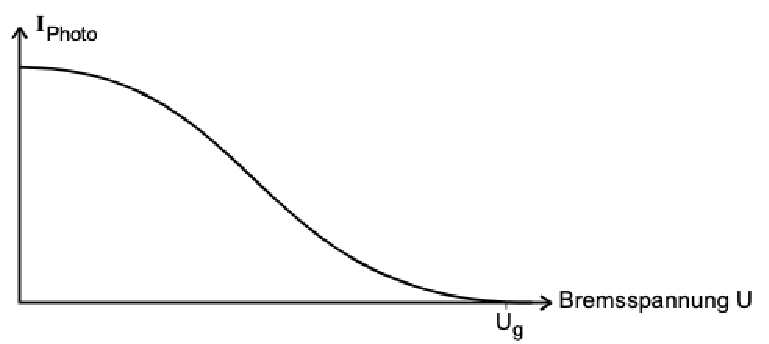
\includegraphics[height=6cm]{content/pics/Photostrom.pdf}
    \caption{Photostrom $I$ in Abhängigkeit von der Bremsspannung $U_{\symup{B}}$ \cite{v500}.}
    \label{fig:Photostrom}
\end{figure}
Dies lässt sich damit erklären, dass die Elektronen bereits vor dem Austritt aus der Photokathode eine Energieverteilung gemäß der
Fermi-Dirac-Statistik haben. Für diesen Versuch ergibt sich in guter Näherung ein quadratischer Zusammenhang zwischen dem Photostrom $I$ und
der Bremsspannung $U_{\symup{B}}$ gemäß
\begin{equation*}
    I \propto U_{\symup{B}}^2.
\end{equation*}
